\chapter{Program Modification}

\section{Search Routines}

During the verification and modification of main programs (\textbf{PM}) and subprograms (\textbf{MM}), search routines allow for the quick location of the desired program blocks.

\subsection{Address Search Routine}

The \textbf{address letter} is the search criterion for the address search routine. This routine automatically finds all program blocks containing a word with the specified address letter.

For example, if it is necessary to verify or modify feed rate parameters (\textbf{F}) in a program, the search routine will find each program block containing a word \textbf{F}, one after the other.

The address search routine allows searching \textbf{forward} and \textbf{backward} in the program.

\procedure

\begin{itemize}
    \item Search for the main program (\textbf{PM}) (see section 6.3.1) or the subprogram (\textbf{MM}) (see section 6.4) that needs to be modified.
\end{itemize}

\begin{itemize}
    \iconitem{Select the desired address letter by using the cursor control keys \textbf{"left-right"}.}{left.jpg,right.jpg}
\end{itemize}

\vspace{.5cm}

\begin{itemize}
    \iconitem{Search for the block by pressing the cursor control key \textbf{"up-down"}.}{up.jpg,down.jpg}
\end{itemize}

\vspace{.5cm}

The upper cursor moves to the next \textbf{block N} in the program that contains a word with the selected address letter.

The found block is displayed on \textbf{line 21} of the screen.

If the program does not contain any block with a word that includes the selected address letter, the screen display remains unchanged.

\notes

After each \textbf{modification} of a program block, the cursor is moved to the address letter \textbf{G}.

If a new block search is to be performed for the next block number, the cursor must first be moved to the address letter \textbf{N}.

\newpage
\underline{\textbf{Address Letter with Equality Sign}}

For an automatic search of program blocks containing a word where the address letter is defined in relation to the \textbf{equality sign}, it is necessary, after selecting the address letter, to enter \textbf{all characters up to and including the equality sign} before the search procedure can be started by pressing one of the cursor control keys \textbf{"up-down"}.

\example

\begin{center}
    \textbf{Example 1:} \fbox{\textbf{E13=150}}
\end{center}

\begin{itemize}
    \item Move the cursor to \textbf{E}.
    \item Enter \textbf{13} using the numeric keypad.
    \item Enter the \textbf{equality sign} by pressing the \textbf{EQUAL} key.
    \item Search for the block by pressing one of the cursor control keys \textbf{"up-down"}.
\end{itemize}

\begin{center}
    \textbf{Example 2:} \fbox{\textbf{N=9001}}
\end{center}

\begin{itemize}
    \item Move the cursor to \textbf{N}.
    \item Enter the \textbf{equality sign} by pressing the \textbf{EQUAL} key.
    \item Search for the block by pressing one of the cursor control keys \textbf{"up-down"}.
\end{itemize}

\notes

If a word in which the address letter is defined in relation to the equality sign is found but \textbf{not modified}, it is necessary to first press the \textbf{CLEAR} key before starting a new search procedure.

\newpage

\subsection{Word Search Routine}

The search criterion for this routine is the \textbf{entire word}.

The search routine automatically finds all program blocks that contain such a word.

With the word search routine, the search procedure within the program can only be performed \textbf{"forward"}.

\procedure

\begin{itemize}
    \item Search for the main program \textbf{PM} (see section 6.3.1) or the subprogram \textbf{MM} (see section 6.4) that needs to be modified.
\end{itemize}

\begin{itemize}
    \iconitem{Select the address letter of the word to be searched by pressing the cursor control keys \textbf{"left-right"}.}{left.jpg,right.jpg}
\end{itemize}

\vspace{.5cm}

\begin{itemize}
    \item Enter the corresponding value using the numeric keypad.
\end{itemize}

\begin{itemize}
    \iconitem{Press the \textbf{ENTER} key.}{enter.jpg}
\end{itemize}

\vspace{.5cm}

\begin{itemize}
    \iconitem{Press the \textbf{SEARCH} key.}{search.jpg}
\end{itemize}

\vspace{.5cm}

The upper cursor jumps to the next \textbf{block N} in the program that contains the entered word.

The found block is displayed on \textbf{line 21} of the screen.

\notes

If no block containing the entered word exists in the program, an error is displayed on \textbf{line 3} of the screen.

\section{Modification of the Active Main Program}

The active main program \textbf{PM actif} is the program displayed on \textbf{line 2} of the screen in all command operation modes.

During program execution, the active main program \textbf{PM} cannot be modified. The same applies to subprograms \textbf{MM}.

However, it is possible to modify all non-active main programs \textbf{PM} while the program is running (see section 6.3).

The active main program \textbf{PM} \textbf{must} be modified in \textbf{MANUAL} mode.

\newpage
\subsection{Searching for the Block to be Modified}

\begin{itemize}
    \iconitem{Press the \textbf{MANUAL} key.}{manual.jpg}
\end{itemize}

\vspace{.5cm}

\begin{itemize}
    \iconitem{Press the \textbf{PROG.MEM.} key.}{prog_mem.jpg}
\end{itemize}

\vspace{.5cm}

The active main program is displayed on the screen:

\begin{center}
    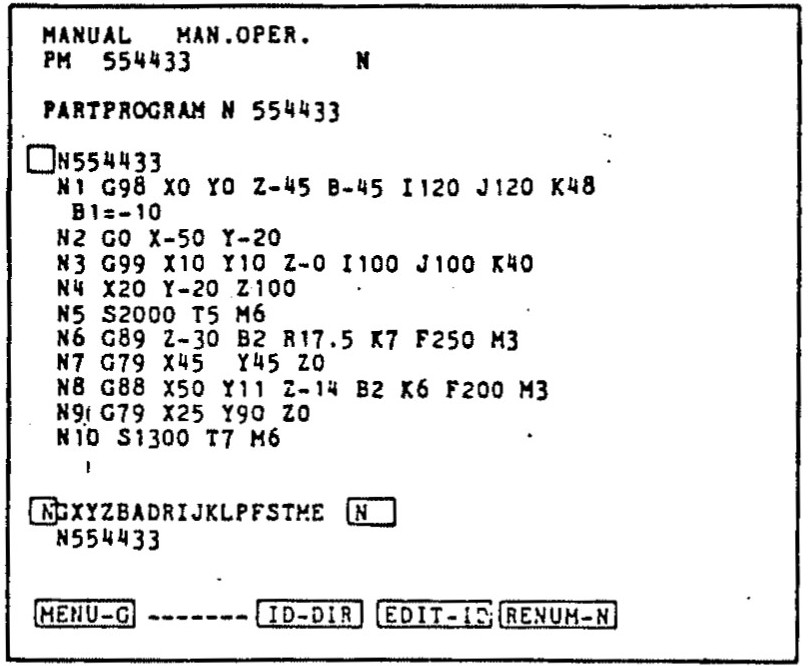
\includegraphics[width=0.8\textwidth]{active_program.jpg}
\end{center}

The cursor is positioned in front of the program number \textbf{N} of the active main program.

There are \textbf{two possibilities} for searching for the block to be modified:

\subsubsection*{First Search Method}

\begin{itemize}
    \iconitem{Move the cursor to the line with the number \textbf{N} of the desired block, using the command keys "up-down".}{up.jpg,down.jpg}
\end{itemize}

The searched block is now also displayed on \textbf{line 21} of the screen.

\subsubsection*{Second Search Method}

\begin{itemize}
    \item Enter the number \textbf{N} of the block to be searched on the numeric keypad.
\end{itemize}

\begin{itemize}
    \iconitem{Press the \textbf{ENTER} key.}{enter.jpg}
\end{itemize}

The entered \textbf{N} block number appears on \textbf{line 21} of the screen.

\begin{itemize}
    \iconitem{Press the \textbf{SEARCH} key.}{search.jpg}
\end{itemize}

The searched block appears in the first position of the program section displayed on the screen.

The searched block is also displayed on \textbf{line 21} of the screen.

The lower cursor on the screen is now positioned at the address letter \textbf{G}.  
It must be moved back to the address letter \textbf{N} if the search procedure needs to continue as described.

\notes

It is always useful to use the \textbf{second search method} if the searched block \textbf{N} is outside the program section displayed on the screen.

\subsection{Modification, Insertion, and Deletion of Program Words}

\begin{itemize}
    \item Search for the program block to be modified (see section 6.2.1).
\end{itemize}

The \textbf{search routines} can be used to locate the block (see sections 6.1.1 and 6.1.2).

\begin{itemize}
    \iconitem{Move the cursor to the address letter of the word to be modified, inserted, or deleted using the command keys "left-right".}{left.jpg,right.jpg}
\end{itemize}

\begin{itemize}
    \item Enter the corresponding numeric value on the numeric keypad if the existing word is to be modified or a new word is to be entered.
\end{itemize}

Do \textbf{not} enter \textbf{any} numeric value if the existing word needs to be deleted.

When deleting a word where the address letter is defined with an equality sign, \textbf{enter all characters including the \texttt{=} sign}.

\begin{itemize}
    \iconitem{Press the \textbf{ENTER} key.}{enter.jpg}
\end{itemize}

Pressing the key causes the modified or inserted word to be displayed on \textbf{line 14} of the screen; a deleted word disappears.

Once all necessary words for the selected program block have been modified, inserted, or deleted:

\begin{itemize}
    \iconitem{Press the \textbf{STORE} key.}{store.jpg}
\end{itemize}

Pressing the \textbf{STORE} key saves the modified block.  
Instead of the old block, the new block is now placed in the program section displayed on the screen.

The next program block appears on \textbf{line 21} of the screen.

If no further modifications to the program are needed:

\begin{itemize}
    \iconitem{Press the \textbf{MANUAL} key.}{manual.jpg}
\end{itemize}

\newpage

\subsection{Deleting a Program Block}

\begin{itemize}
    \item Search for the program block to be modified (see section 6.2.1).
\end{itemize}

\begin{itemize}
    \iconitem{Move the cursor to the address letter \textbf{N} by using the command keys "left-right".}{left.jpg,right.jpg}
\end{itemize}

\vspace{.5cm}

\begin{itemize}
    \iconitem{Press the \textbf{ENTER} key.}{enter.jpg}
\end{itemize}

\vspace{.5cm}

The selected block number \textbf{N}, followed by the complement (\textbf{CLEAR}), is displayed on \textbf{line 21} of the screen.

\begin{itemize}
    \iconitem{Press the \textbf{STORE} key.}{store.jpg}
\end{itemize}

\vspace{.5cm}

Pressing the \textbf{STORE} key deletes the program block.  
It disappears from the displayed program section on the screen.

If no further modifications to the program are needed:

\begin{itemize}
    \iconitem{Press the \textbf{MANUAL} key.}{manual.jpg}
\end{itemize}

\vspace{.5cm}

\subsection{Inserting a Program Block}

It is possible to insert new blocks at any point in the program.

\begin{itemize}
    \item Search for the block \textbf{after which} the new block should be inserted in the program (see section 6.2.1).
\end{itemize}

\begin{itemize}
    \iconitem{Move the cursor to the address letter \textbf{N} by using the command keys "left-right".}{left.jpg,right.jpg}
\end{itemize}

\vspace{.5cm}

\begin{itemize}
    \item Enter the sequence number \textbf{N} to be inserted using the numeric keypad.
\end{itemize}

This sequence number \textbf{must not} already exist in the program.

\begin{itemize}
    \iconitem{Press the \textbf{ENTER} key.}{enter.jpg}
\end{itemize}

\vspace{.5cm}

\begin{itemize}
    \iconitem{Move the cursor to the corresponding address letter using the command keys "left-right".}{left.jpg,right.jpg}
\end{itemize}

\begin{itemize}
    \item Enter the numerical value using the numeric keypad.
\end{itemize}

\begin{itemize}
    \iconitem{Press the \textbf{ENTER} key after each program word formed according to the described procedure (address letter + numerical value).}{enter.jpg}
\end{itemize}

\begin{itemize}
    \iconitem{Press the \textbf{STORE} key after entering all words for the block to be inserted.}{store.jpg}
\end{itemize}

\vspace{.5cm}

Pressing the \textbf{STORE} key saves the new block and inserts it into the program section displayed on the screen.

If no further modifications need to be made to the program:

\begin{itemize}
    \iconitem{Press the \textbf{MANUAL} key.}{manual.jpg}
\end{itemize}

\newpage

\section{Modifying a Non-Active Main Program}

The main program \textbf{PM} displayed on \textbf{line 2} of the screen in all command operation modes is the active main program.  
All other programs listed with their program numbers are \textbf{non-active main programs}.

Non-active main programs can be modified even while the machine's program is \textbf{running}.

\subsection{Searching for the Program to be Modified}

\begin{itemize}
    \iconitem{Press the \textbf{PROG.MEM} key.}{prog_mem.jpg}
\end{itemize}

The active main program appears on the screen:

\begin{itemize}
    \iconitem{Press the \textbf{F3} function key (ID-DIR).}{f3.jpg}
\end{itemize}

\begin{center}
    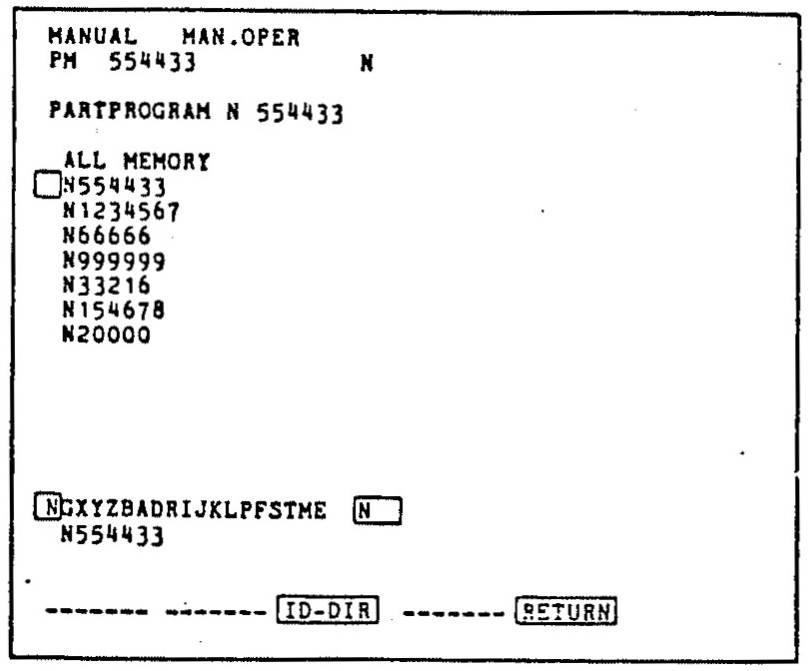
\includegraphics[width=0.7\textwidth]{program_list.jpg}
\end{center}

The list of program numbers stored in memory appears on the screen.

There are \textbf{two possibilities} for searching the non-active main program \textbf{PM} to be modified:

\subsubsection*{First Search Option}

\begin{itemize}
    \item Move the cursor to the line with the program number \textbf{N} by using the command keys \textbf{"up and down"}.
\end{itemize}

\begin{itemize}
    \iconitem{Press the \textbf{SEARCH} key.}{search.jpg}
\end{itemize}

The first blocks of the program to be modified appear on the screen.
\newpage
\subsubsection*{Second Search Option}

\begin{itemize}
    \item Enter the program number \textbf{N} to be searched using the numeric keypad.
\end{itemize}

\begin{itemize}
    \iconitem{Press the \textbf{ENTER} key.}{enter.jpg}
\end{itemize}
\vspace{.5cm}
The entered program number \textbf{N} appears on \textbf{line 21} of the screen.

\begin{itemize}
    \iconitem{Press the \textbf{SEARCH} key.}{search.jpg}
\end{itemize}
\vspace{.5cm}
The first blocks of the program to be modified appear on the screen.

\begin{center}
    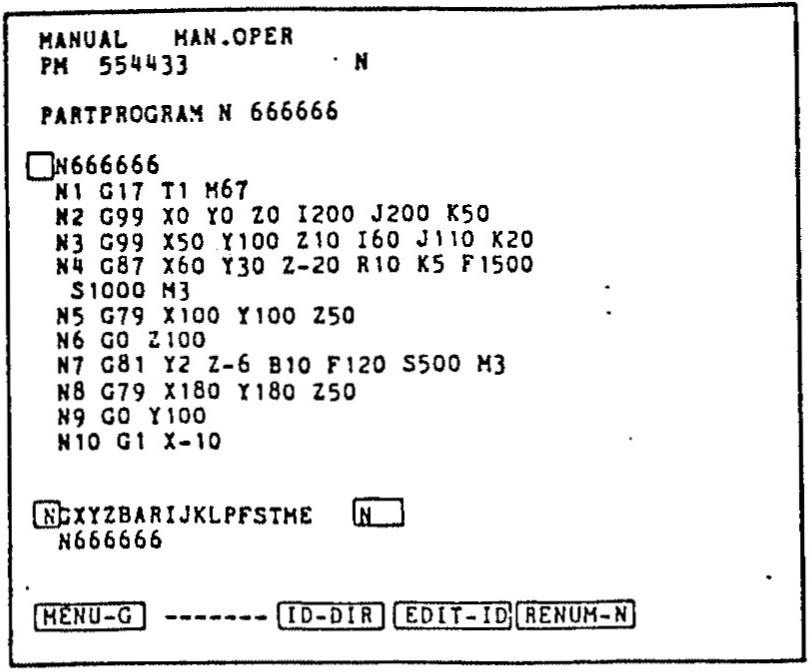
\includegraphics[width=0.7\textwidth]{program_blocks.jpg}
\end{center}
\notes

It is always useful to use the \textbf{second search option} if the program number \textbf{N} being searched is outside the list of program numbers in the main program memory displayed on the screen.

The active main program is displayed as before at \textbf{line 2} of the screen.

The non-active main program to be modified is displayed at \textbf{line 4} of the screen.

\underline{\textbf{Modifying a non-active program}} must be done in the same way as described in section \textbf{6.2} for the active main program.

\begin{itemize}
    \item \textbf{Modification, insertion, and deletion of program words}, see section \textbf{6.2.2}.
    \item \textbf{Deleting a program block}, see section \textbf{6.2.3}.
    \item \textbf{Inserting a program block}, see section \textbf{6.2.4}.
\end{itemize}

After modifying a non-active main program \textbf{P}:

\begin{itemize}
    \iconitem{Press the \textbf{MANUAL}, \textbf{TEACH IN}, \textbf{SINGLE}, or \textbf{AUTO} key according to the signal displayed on line \textbf{1} of the screen (MANUAL, TEACH IN, SINGLE, or AUTO).}{manual.jpg, teach_in.jpg, single.jpg, auto.jpg}
\end{itemize}

\vspace{1.5cm}

Pressing the appropriate key updates the display on the screen with the selected operating mode.

\section{Modification of Subprograms}

In principle, subprograms (\textbf{MACROS}) must be modified in \textbf{MANUAL} mode.

\procedure

\begin{itemize}
    \iconitem{Press the \textbf{MANUAL} key.}{manual.jpg}
\end{itemize}
\vspace{.5cm}
\begin{itemize}
    \iconitem{Press the \textbf{PROG.MEM} key.}{prog_mem.jpg}
\end{itemize}
\vspace{.5cm}
The active main program appears on the screen.

\begin{itemize}
    \iconitem{Press the \textbf{MENU} key.}{menu.jpg}
\end{itemize}
\vspace{.5cm}
The \textbf{PROGRAM MENU} appears on the screen:

\begin{center}
    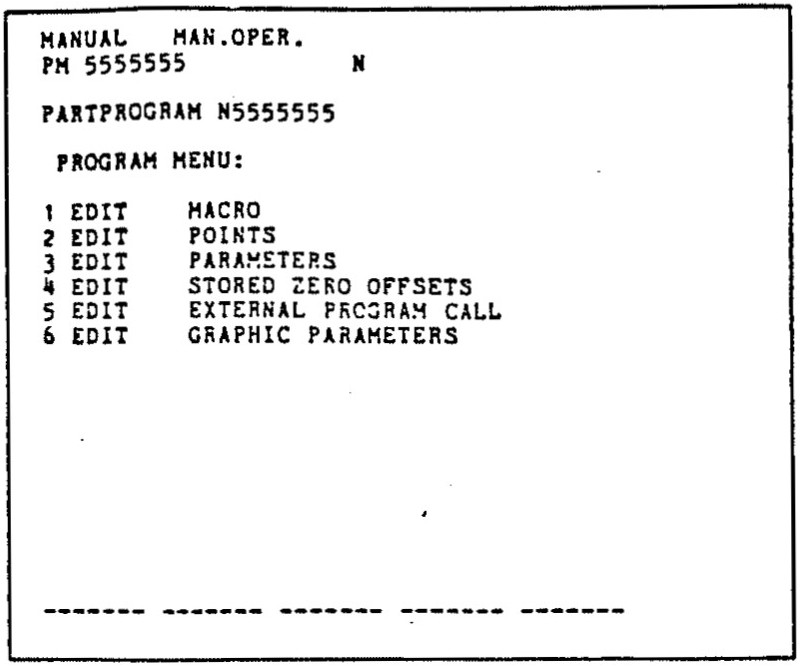
\includegraphics[width=0.7\textwidth]{program_menu.jpg}
\end{center}

\begin{itemize}
    \item Enter the number \textbf{1} on the numeric keypad.
\end{itemize}

The screen now displays the list of subprogram numbers stored in memory.

The subprogram to be modified must be searched using the procedure described in section \textbf{6.3.1} (see the \textbf{first} or \textbf{second search option}).

\underline{\textbf{Modification of subprograms}} must be done in the same way as described in section \textbf{6.2} for the active main program.

\textbf{Modification, insertion, and deletion of program words}, see section \textbf{6.2.2}.

\textbf{Erasing a program block}, see section \textbf{6.2.3}.  

\textbf{Inserting a program block}, see section \textbf{6.2.4}.

Once modifications to a subprogram \textbf{MM} are complete:

\begin{itemize}
    \iconitem{Press the \textbf{MANUAL} key.}{manual.jpg}
\end{itemize}

\newpage

\section{Program Erasure}

The active main program and subprograms can only be modified in \textbf{MANUAL} mode.  
Non-active main programs can be erased even while the machine is executing a program.

\subsection{Erasing a Single Program}

\procedure

Search for the main program to be erased according to the description in section \textbf{6.3.1} (\textit{see first search option}),  
    or search for the subprogram to be erased according to the description in section \textbf{6.4}.

\begin{itemize}
    \iconitem{Press the \textbf{ENTER} key.}{enter.jpg}
\end{itemize}

The selected program number \textbf{N}, followed by the \textbf{CLEAR} complement, is displayed on line 21 of the screen.

\begin{itemize}
    \iconitem{Press the \textbf{STORE} key.}{store.jpg}
\end{itemize}

Pressing the \textbf{STORE} key deletes the \textbf{separate program}.  
It disappears from the list of program numbers in the main program memory or subprogram memory.

If no further modifications are needed to the main program or subprogram memory:

\begin{itemize}
    \iconitem{Press the \textbf{MANUAL}, \textbf{TEACH IN}, \textbf{SINGLE}, or \textbf{AUTO} key according to the signal displayed on \textbf{line 1} of the screen (MANUAL, TEACH IN, SINGLE, or AUTO).}{manual.jpg, teach_in.jpg, single.jpg, auto.jpg}
\end{itemize}

\vspace{.5cm}

Pressing the appropriate key updates the screen display with the selected operating mode.

\subsection{Erasing All Programs}

\begin{itemize}
    \iconitem{Press the \textbf{MANUAL} key.}{manual.jpg}
\end{itemize}

\vspace{.5cm}

\textbf{Selecting the Main Program Memory}  
See section \textbf{6.3.1}.

\textbf{Selecting the Subprogram Memory}  
See section \textbf{6.4}.

The screen will display the list of program numbers stored in the main program memory or subprogram memory.

\begin{itemize}
    \iconitem{Move the cursor to the \textbf{ALL MEMORY} line using the cursor control keys \textbf{"up-down"}.}{up.jpg,down.jpg}
\end{itemize}

\vspace{.5cm}

\begin{itemize}
    \iconitem{Press the \textbf{ENTER} key.}{enter.jpg}
\end{itemize}

\vspace{.5cm}

The display shows \textbf{ALL MEMORY} on \textbf{line 21}, followed by the complement \textbf{CLEAR}.

\begin{itemize}
    \iconitem{Press the \textbf{STORE} key.}{store.jpg}
\end{itemize}

\vspace{.5cm}

Pressing the \textbf{STORE} key deletes all programs.  
All program numbers are erased from the list of stored programs in the main program memory or subprogram memory.

If, after erasing, no further entries should be made to the main program or subprogram memory:

\begin{itemize}
    \iconitem{Press the \textbf{MANUAL} key.}{manual.jpg}
\end{itemize}

\section{Modification of Program Numbers}

The modification of program numbers can be performed in both the main program memory and the subprogram memory.

Select the memory of the main program (see section \textbf{6.3.1}) or the subprogram memory (see section \textbf{6.4}).

\procedure

\begin{itemize}
    \iconitem{Move the cursor to the program number to be modified using the \textbf{"up-down"} command keys.}{up.jpg,down.jpg}
\end{itemize}

\vspace{.5cm}

\begin{itemize}
    \iconitem{Press the \textbf{SEARCH} key.}{search.jpg}
\end{itemize}

\vspace{.5cm}

\begin{itemize}
    \item Move the cursor to the program number.
\end{itemize}

Enter the new program number using the numeric keypad.

\begin{itemize}
    \iconitem{Press the \textbf{ENTER} key.}{enter.jpg}
\end{itemize}

\vspace{.5cm}

\begin{itemize}
    \iconitem{Press the \textbf{F4} function key (EDIT-ID).}{f4.jpg}
\end{itemize}

\vspace{.5cm}

If no further modifications are required:

\begin{itemize}
    \iconitem{Press the \textbf{MANUAL} key.}{manual.jpg}
\end{itemize}

\vspace{.5cm}

\textbf{Attention:}  
If the program number is modified, this same number must also be updated in the call block (\textbf{G22}) of the main program.

\section{New Sequential Numbering After Block Insertion or Deletion}

This applies not only to main programs but also to subprograms.

\textbf{Selection of Memory:}  
Choose either the \textbf{PM} (main program memory) or the \textbf{MM} (subprogram memory)  
(see procedure described in section \textbf{6.5.1}).

\textbf{Block Insertion:}  
Follow the procedure described in section \textbf{6.2.4}.

\begin{itemize}
    \iconitem{Press the \textbf{F5} function key (RENUM-N).}{f5.jpg}
\end{itemize}

The program blocks are now newly numbered in sequence.

\vspace{.5cm}

If no further modifications are required:

\begin{itemize}
    \iconitem{Press the \textbf{MANUAL} key.}{manual.jpg}
\end{itemize}

\vspace{.5cm}

\notes

Block numbers are also automatically updated in case of repetitive functions (\textbf{G14}).